
\documentclass{abgabe}
\begin{document}

\begin{questions}
    \qformat{\thequestion. \textbf{\thequestiontitle} \hfill}
    \titledquestion{Veranstaltungsverwaltungssystem}

    Gegeben sei folgende Beschreibung für ein Veranstaltungsverwaltungssystem:

    Personen haben Zeichenketten als Name.
    Studenten sind Personen, erben also die Eigenschaften von Person, haben aber zusätzlich eine ganzzahlige Matrikelnummer und nehmen an beliebig vielen Veranstaltungen teil.
    Eine Veranstaltung hat potentiell beliebig viele Teilnehmer, wird aber von einem, zwei oder drei Mitarbeitern betreut.
    Eine Veranstaltung hat eine Veranstaltungsnummer und einen Titel.
    Seminare und Vorlesungen sind spezielle Veranstaltungen.
    Ein Seminar hat eine begrenzte Anzahl an Plätzen, für eine Vorlesung wird eine Klausur angeboten oder nicht.
    Mitarbeiter sind Personen und betreuen eine bis fünf Veranstaltungen und haben eine Personalnummer.
    Professoren und Assistenten sind Mitarbeiter.
    Assistenten sind bei genau einem Professor beschäftigt und haben eine bestimmt Finanzierung (Zeichenkette).
    Ein Professor hat ein Lehrgebiet (Zeichenkette), beschäftigt beliebig viele Assistenten und ist Inhaber von genau einem Lehrstuhl.
    Ein Lehrstuhl hat eine Bezeichnung und genau einen Professor als Inhaber.

    Erstellen Sie anhand der obigen Beschreibung ein \emph{Klassendiagramm}.
    Ihr Diagramm sollte folgende Punkte beinhalten:
    \begin{itemize}
        \item \emph{Generalisierungsbeziehungen},
        \item \emph{Assoziationen} mit Assoziationsnamen und Leserichtung,
        \item \emph{Multiplizitäten} sowie
        \item \emph{Attributnamen} und (sinnvolle) \emph{–typen}.
    \end{itemize}

    Finden Sie jeweils ein Beispiel, bei dem eine Aggregations- und eine Kompositionsbeziehung sinnvoll ist.
    Erläutern Sie kurz den Unterschied zwischen Aggretation und Komposition anhand des Bespiels.
    \begin{solution}
        \begin{center}
            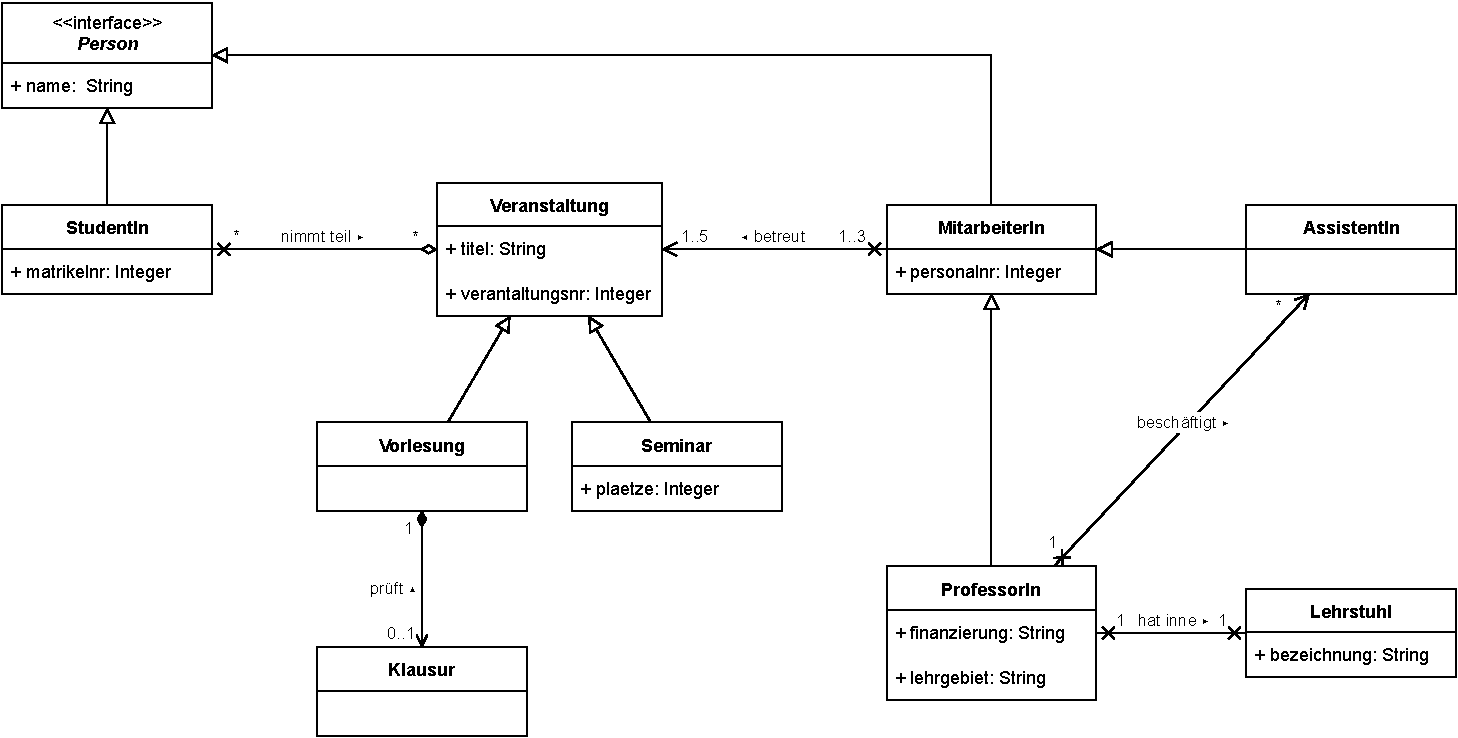
\includegraphics[width=.75\textwidth]{swt_h07_veranstaltungsverwaltung.pdf}
        \end{center}
    \end{solution}
\end{questions}
\end{document}